% ============================================================
% Amazon-VT CFP 2026-2027 — 1-Page Abstract v4b
% AKG-E Reframed: 2 Applications + VVUQ as core contribution
% Primary: AI Accelerated Science & Engineering
% Secondary: Agentic AI
% Format: IEEE 2-column
% ============================================================

\documentclass[conference, 10pt]{IEEEtran}

\usepackage[utf8]{inputenc}
\usepackage[T1]{fontenc}
\usepackage{graphicx}
\usepackage{hyperref}
\usepackage{microtype}
\usepackage{cite}
\usepackage{enumitem}
\setlist{nosep, leftmargin=1.5em, topsep=0.2em}
\usepackage{tikz}
\usetikzlibrary{positioning, arrows.meta, shapes.geometric, fit, calc}

\title{Agentic Knowledge Graphs with Simulation-in-the-Loop\\VVUQ for Construction and Transportation Engineering}
\author{}
\date{}

% ============================================================
\begin{document}

\maketitle
\thispagestyle{empty}

\vspace{-1.5em}

\noindent\textbf{Primary Topic:} AI Accelerated Science \& Engineering \hfill
\textbf{Secondary:} Agentic AI

\vspace{0.5em}

AI-driven scientific breakthroughs---from biomolecular structure prediction~\cite{Abramson2024AlphaFold3} to materials discovery~\cite{Merchant2023GNoME}---demonstrate that domain-specific AI can dramatically accelerate discovery when tightly coupled to structured domain knowledge and simulation. Engineering disciplines face an analogous opportunity, yet large language models remain poorly suited to engineering practice: they hallucinate physical quantities~\cite{Ji2023HallucinationSurvey}, cannot enforce constraint satisfaction, and lack grounding in the structured ontologies and simulation feedback loops that define engineering workflows. Meanwhile, physics-informed machine learning~\cite{Karniadakis2021PINN} and digital twin architectures~\cite{Tao2019DigitalTwin} have matured in isolation from generative AI, creating an integration gap between simulation-based engineering and the emerging agentic paradigm.

This project proposes \textbf{Agentic Knowledge Graph Engineering (AKG-E)}, a framework that enables LLM-powered agents to reason over structured engineering knowledge, interact with physics-based simulations, and validate outputs through \textbf{Verification, Validation, and Uncertainty Quantification (VVUQ)}~\cite{Oberkampf2010VVUQ}. While VVUQ is well-established for computational simulation models, no methodology exists for systematically validating AI agent-generated engineering outputs---creating a critical trust gap that blocks deployment. AKG-E addresses this through three layers: (1)~a \textit{domain ontology layer} encoding engineering knowledge graphs (KGs) with entities, constraints, physical laws, and design rules; (2)~a \textit{simulation integration layer} exposing domain tools (finite element analysis solvers, microsimulators) as agent-callable interfaces; and (3)~a \textit{VVUQ validation layer} that verifies agent-generated designs against physical laws, quantifies prediction uncertainty via Monte Carlo propagation through agent pipelines, and enforces regulatory constraints. Agents orchestrate across retrieval-augmented generation~\cite{Lewis2020RAG}, structured graph queries~\cite{Edge2024GraphRAG}, and simulation calls based on task requirements.

\begin{figure}[t]
    \centering
    \resizebox{\columnwidth}{!}{%
    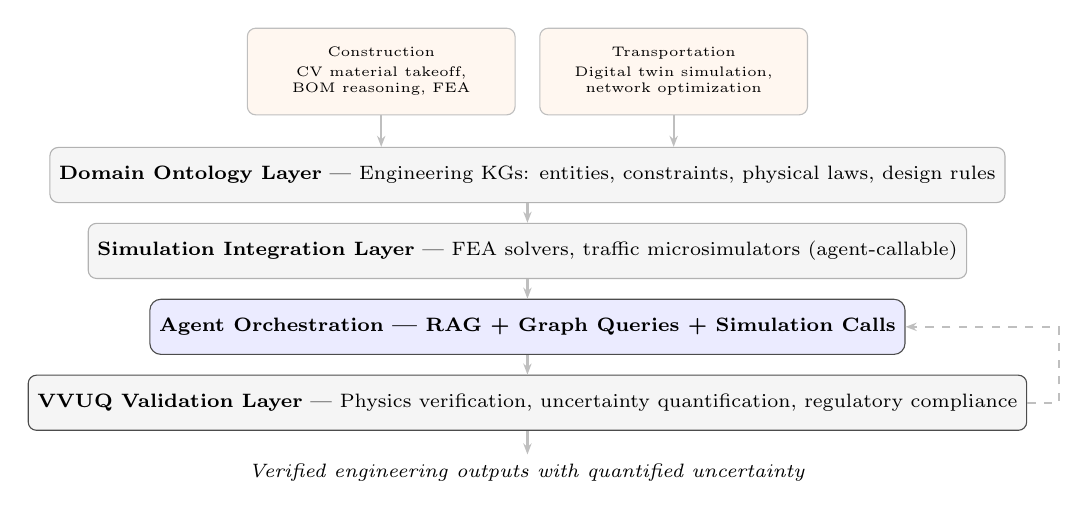
\begin{tikzpicture}[
        node distance=0.35cm and 0.25cm,
        layerbox/.style={rectangle, rounded corners=3pt, draw=gray!60, fill=gray!8, minimum width=7.5cm, minimum height=0.7cm, align=center, font=\scriptsize},
        dombox/.style={rectangle, rounded corners=3pt, draw=gray!50, fill=orange!6, minimum width=3.4cm, minimum height=1.1cm, align=center, font=\tiny},
        agentbox/.style={rectangle, rounded corners=4pt, draw=black!70, fill=blue!8, minimum width=7.5cm, minimum height=0.7cm, align=center, font=\scriptsize\bfseries},
        arr/.style={-{Stealth[length=4pt]}, thick, gray!50},
    ]
        % Domain applications (top) - 2 focused domains
        \node[dombox] (con) {Construction\\[1pt]\tiny CV material takeoff,\\BOM reasoning, FEA};
        \node[dombox, right=0.3cm of con] (traf) {Transportation\\[1pt]\tiny Digital twin simulation,\\network optimization};

        % Domain ontology layer
        \node[layerbox, below=0.4cm of $(con.south)!0.5!(traf.south)$] (onto) {\textbf{Domain Ontology Layer} --- Engineering KGs: entities, constraints, physical laws, design rules};

        % Simulation integration layer
        \node[layerbox, below=0.25cm of onto] (sim) {\textbf{Simulation Integration Layer} --- FEA solvers, traffic microsimulators (agent-callable)};

        % Agent orchestration
        \node[agentbox, below=0.25cm of sim] (agent) {Agent Orchestration --- RAG + Graph Queries + Simulation Calls};

        % VVUQ validation
        \node[layerbox, below=0.25cm of agent, draw=black!70] (val) {\textbf{VVUQ Validation Layer} --- Physics verification, uncertainty quantification, regulatory compliance};

        % Output
        \node[font=\scriptsize, below=0.3cm of val] (out) {\textit{Verified engineering outputs with quantified uncertainty}};

        % Arrows
        \draw[arr] (con.south) -- (con.south |- onto.north);
        \draw[arr] (traf.south) -- (traf.south |- onto.north);
        \draw[arr] (onto) -- (sim);
        \draw[arr] (sim) -- (agent);
        \draw[arr] (agent) -- (val);
        \draw[arr] (val) -- (out);

        % Feedback loop
        \draw[arr, dashed] (val.east) -- ++(0.4,0) |- (agent.east);
    \end{tikzpicture}
    }%
    \caption{\textbf{AKG-E Framework with VVUQ.} Two engineering domains plug into shared ontology, simulation, and validation layers. Agents orchestrate retrieval, graph reasoning, and simulation calls. The VVUQ layer verifies outputs, quantifies uncertainty, and enforces constraints. A feedback loop ensures iterative refinement until validation criteria are met.}
    \label{fig:framework}
    \vspace{-0.5em}
\end{figure}

The framework is demonstrated through two applications sharing the VVUQ backbone. In \textbf{construction engineering}, agents perform automated material takeoff using computer vision, reason over bill-of-materials knowledge graphs grounded in BIM/IFC standards, and validate structural designs through FEA---with VVUQ ensuring load calculations satisfy building codes and quantifying safety margins. In \textbf{transportation engineering}, agents build and query digital twin models~\cite{Tao2019DigitalTwin} of traffic networks, optimize signal timing, and validate proposals through microsimulation---with VVUQ verifying flow capacity constraints and quantifying prediction uncertainty under varying demand. Both applications exercise the same three-layer architecture; only the domain ontology and simulation interfaces differ.

This research tests two hypotheses: \textbf{H1:}~Agents grounded in engineering KGs with simulation-in-the-loop VVUQ produce significantly fewer physically infeasible outputs than RAG-only or prompt-only LLM baselines on engineering tasks (target: $>$50\% constraint violation reduction). \textbf{H2:}~VVUQ-aware agent pipelines yield calibrated uncertainty estimates for engineering quantities (coverage within 10\% of nominal), enabling principled confidence thresholds for autonomous versus human-reviewed decisions.

Experiments compare prompt-only LLMs, RAG-augmented methods, and full AKG-E on construction (material takeoff, BOM validation, structural verification) and transportation (digital twin optimization, network design) tasks. Expected outcomes include the open AKG-E framework, VVUQ-integrated KG templates, and benchmarks demonstrating that \textbf{simulation-grounded agentic AI} outperforms unstructured approaches for engineering decision-support.

\bibliographystyle{IEEEtran}
\bibliography{references}

\end{document}
